\clearpage
\section{Analysis of 2D linear systems}
\begin{colbox}
    \begin{description}
        \item[Part 1: Direct analysis.] For each of the following 2D linear systems with \(\vb{\dot{x}}=A\vb{x}\), compute the eigenvalues and (when real) the eigenvectors of \(A\), and sketch the phase portrait. Indicate the directions of the eigenvectors when real, the sense of rotation when complex, and a few representative trajectories. \begin{enumerate}
            \item \(\dot{x}=x+3y, \quad \dot{y}=2x\)
            \item \(\dot{x}=-2x-4y,\quad \dot{y}=x-2y\)
        \end{enumerate}
        \item[Part 2: Classification from trace and determinant alone.] For the matrix below, classify the fixed point at the origin using only \(T=\tr A\) and \(\Delta = \det A\). No need to copmute the eigenvalues explicitly.\begin{equation}
            A = \mqty(-3 & 1 \\ 2 & -4)
        \end{equation}
    \end{description}
\end{colbox}
\subsection{Direct analysis}
\subsubsection{first one}
rewriting into matrix form 
\begin{equation}
    A = \mqty(1&3\\2&0)
\end{equation}
We find the eigenvalues
\begin{align}
    \det\mqty(1-\lambda & 3\\2&-\lambda) = \lambda\ins{\lambda-1}-6=\lambda^2-\lambda-6 = \ins{\lambda-3}\ins{\lambda+2}=0
\end{align}
giving us the eigenvalues 
\begin{align}
    \lambda = 3 && \lambda = -2
\end{align}
and to find the eigenvectors 
\begin{equation}
    \mqty(-2 & 3\\2&-3)v = 0 \implies v=\mqty(3\\2)
\end{equation}
for \(\lambda = 3\), meaning trajectories move outwards along this vector and 
\begin{equation}
    \mqty(3 & 3\\2&2)v=0 \implies v=\mqty(1\\-1)
\end{equation}
for \(\lambda = -2\), meaning trajectories move inwards along this vector.
\subsubsection{second one}
Again 
\begin{equation}
    A = \mqty(-2 & -4 \\ 1 & -2)
\end{equation}
with eigenvalues 
\begin{equation}
    \det\mqty(-2-\lambda&-4\\1&-2-\lambda)=\ins{2+\lambda}^2+4=\lambda^2+4\lambda+8=0
\end{equation}
therefore 
\begin{equation}
    \lambda_{1,2}=\frac{-4\pm\sqrt{16-32}}{2} = \frac{-4\pm4i}{2}=-2\pm2i
\end{equation}
now if we plug in, for example, \(x=1, y=0\) we get 
\begin{align}
    \dot{x} = -x && \dot{y}=1
\end{align}
meaning this would move up and to the left, implying a counter clockwise rotation spiral inwards.
\subsubsection{Figures}
\begin{figure}[!h]
    \begin{subfigure}{0.48\textwidth}
        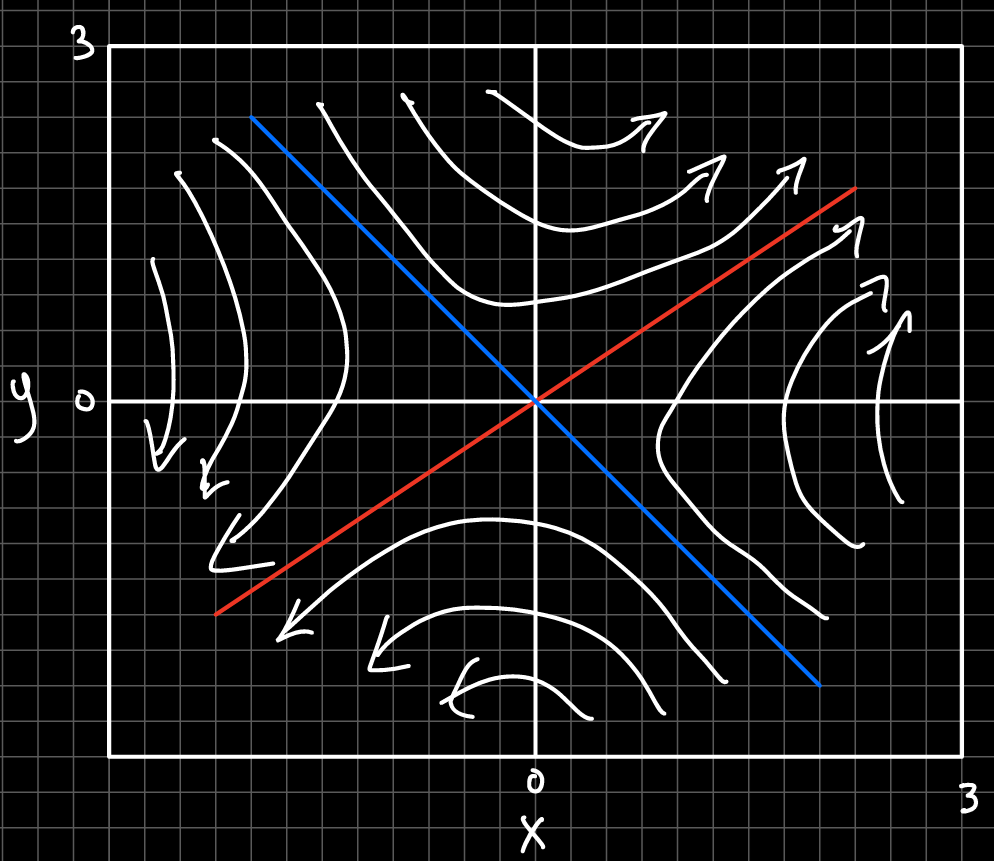
\includegraphics[width=\textwidth]{Untitled.png}
        \caption{Saddle, \(\lambda =3, -2\)}
    \end{subfigure}
    \begin{subfigure}{0.48\textwidth}
        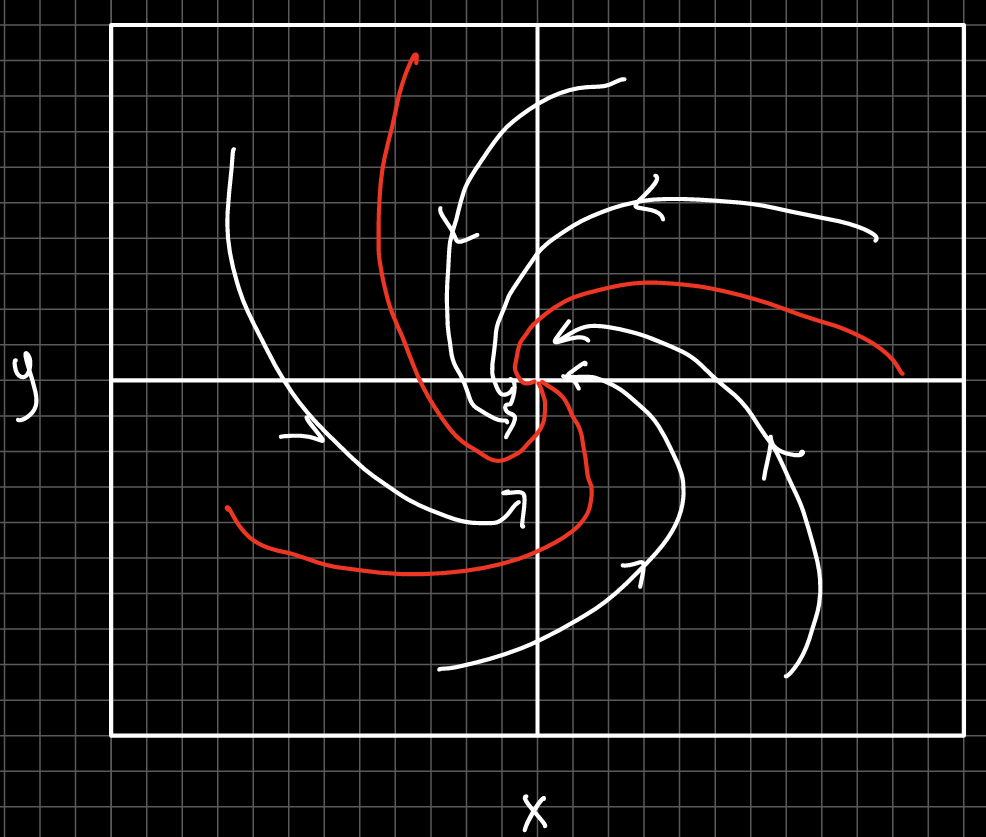
\includegraphics[width=\textwidth]{Untitled2.png}
        \caption{Stable spiral, \(\lambda = -2\pm2i\)}
    \end{subfigure}
\end{figure}
\subsection{Classification}
The trace and determinant are 
\begin{equation}
    \tr A = -7 \qquad \det A = 10
\end{equation}
therefore the discriminant is 
\begin{equation}
    \tr^2-4\Delta = 49-40=9>0
\end{equation}
meaning there are two real distinct eigenvalues. A positive determinant means they share a sign and the negative trace makes the sign negative. Therefore the origin is a stable node.